\documentclass[]{include/latex-class-ceurart/ceurart}

\usepackage[utf8]{inputenc}
\usepackage{amsmath}
\usepackage{amssymb}
\usepackage{microtype}
\usepackage{url}\urlstyle{tt}
\usepackage{bm}
\usepackage{wrapfig}

\usepackage{include/macros/listings}

\input{include/flatland/flatland}
\usetikzlibrary{shapes, arrows, positioning}

\input{include/macros/systems}
\newcommand{\flaspland}{\sysfont{flaspland}}
\newcommand{\Flaspland}{\sysfont{Flaspland}}
%\lstset{xleftmargin=2\parindent,aboveskip=\smallskipamount,belowskip=\smallskipamount,captionpos=b}
%\lstset{numbers=left,numberblanklines=false,basicstyle=\ttfamily}

%\lstdefinelanguage{clingos}{%
 % language=clingo,%
%  basicstyle=\small\ttfamily%
%}
%\makeatletter\lst@AddToHook{OnEmptyLine}{\vspace{\dimexpr-\baselineskip+\medskipamount\relax}}\makeatother

%\newcommand{\positionFunc}{\ensuremath{p}}
\newcommand{\typeFunc}{\ensuremath{t}}
\newcommand{\neighborFunc}{\ensuremath{a}}

\newcommand{\type}[1]{\ensuremath{\typeFunc(#1)}}
\newcommand{\neighbor}[2]{\ensuremath{\neighborFunc(#1,#2)}}

\newcommand{\startFunc}{\ensuremath{s}}
\newcommand{\goalFunc}{\ensuremath{g}}
\newcommand{\orientationFunc}{\ensuremath{o}}
\newcommand{\departFunc}{\ensuremath{\delta}}
\newcommand{\arriveFunc}{\ensuremath{\alpha}}

\newcommand{\start}[1]{\ensuremath{\startFunc(#1)}}
\newcommand{\goal}[1]{\ensuremath{\goalFunc(#1)}}
\newcommand{\orientation}[1]{\ensuremath{\orientationFunc(#1)}}
\newcommand{\depart}[1]{\ensuremath{\departFunc(#1)}}
\newcommand{\arrive}[1]{\ensuremath{\arriveFunc(#1)}}

\newcommand{\forward}{\ensuremath{f}}
\newcommand{\lefturn}{\ensuremath{l}}
\newcommand{\righturn}{\ensuremath{r}}
\newcommand{\wait}{\ensuremath{w}}

\newcommand{\resultFunc}{\ensuremath{d}}
\newcommand{\preconditionFunc}{\ensuremath{p}}

\newcommand{\result}[1]{\ensuremath{\resultFunc(#1)}}
\newcommand{\precondition}[1]{\ensuremath{\preconditionFunc(#1)}}

\newcommand{\connected}[1]{%
  \mathrel{\vbox{\offinterlineskip\ialign{%
    \hfil##\hfil\cr%
    $\scriptstyle\mathit{#1}$\cr%
    \noalign{\kern1pt}%
    $\hookrightarrow$\cr%
    \noalign{\kern-0.1pt}%
}}}}
%%% Local Variables:
%%% mode: LaTeX
%%% TeX-master: "paper"
%%% End:

%\newcommand{\notation}[1]{\par\smallskip\noindent\textbf{Notation.}{\em~#1}\par}
%\newtheorem{proposition}{Proposition}

% \usepackage{comments}

\begin{document}
\conference{22nd Doctoral Consortium (DC) on Logic Programming}

\title{ICLP-DC-SS-2026: \\ Modeling Railway Systems in Answer Set Programming}

\author[1]{Ryan Murphy}[email=ryan.murphy@uni-potsdam.de]
\address[1]{University of Potsdam, Germany}

\maketitle

\begin{abstract}
\flaspland
\end{abstract}

\section{Introduction}\label{sec:introduction}

\begin{figure}[ht]
  \centering
  \includegraphics[width=0.60\linewidth, keepaspectratio]{figures/example-small.png}
  \caption{An example Flatland railway environment.}
  \label{fig:environment}
\end{figure}

Railway systems face numerous operational challenges in planning and execution,
and have been the subject of research for decades, particularly since the middle of the twentieth century.
By 2002, it was proven that developing train timetables for a single track belongs to the class NP-Hard \cite{}.
As modern railway systems grow,
both in terms of their networks and their passenger demand,
the real problems they face become more complex
and require more advanced solutions.

Tasked with solving such complex issues
and inspired by advancements in digital technology,
the Swiss Federal Railway (SBB) founded \textit{Flatland},
a global online railway scheduling and rescheduling competition
to crowdsource novel approaches to modern-day problems.
An example Flatland environment is shown in Figure~\ref{fig:environment}.
My research began in 2023 as an attempt to use answer set programming (ASP)
as an alternative to the machine learning approaches.
This culminated in a master thesis that outlined the creation of a toolkit
now known as \textit{flaspland}
that provides an interface between \textit{Flatland} written in Python
and ASP written in clingo.
The work also established standard fact formats for representing railway environments
and put forth simple baseline encodings for safely navigating trains.

The research continues today in the form of Ph.D. work
under the supervision of Prof. Dr. Torsten Schaub,
and includes a graduate-level railway scheduling course,
where students explore solutions to open research topics in this area,
and theses written by highly-motivated students
with a particular affinity for
research at the intersection between
knowledge representation and public transportation.
In this paper, I will: 
provide \textbf{background context} into the history of railway research, modern approaches, and the advantages of answer set programming; 
outline my \textbf{research goals} for the next few years; 
highlight the \textbf{current status} of this research;
share some \textbf{preliminary results};
and bring attention to \textbf{milestones} that lie on the horizon.


%
%%% Local Variables:
%%% mode: LaTeX
%%% TeX-master: "paper"
%%% End:

\section{Background}\label{sec:background}

\begin{enumerate}
	\item Research into railway operations began back in \dots
	\item Answer set programming has tackled problems in similar domains, such as multi-agent pathfinding, airline and traffic management, etc.
	\begin{enumerate}
		\item The hybrid railway scheduling paper for SBB (cite and expand)
		\item Some of Klaus's papers for MAPF
		\item Alice's Traffic Signal paper from TAASP
		\item Alexander's Air Traffic Flow work on capacity
	\end{enumerate}
\end{enumerate}

%
%%% Local Variables:
%%% mode: LaTeX
%%% TeX-master: "paper"
%%% End:

\section{Research goals}\label{sec:goal}

The goal of this research is to establish best practices for modeling large railway systems in answer set programming.
Our initial goal has been to understand large railway systems by leveraging the virtual railway environment generator, Flatland.
In doing so, developing a comprehensive formalization of the problem, as well as initial encodings, has enabled us to see how the problem of railway management differs from those in similar domains.
Ultimately, this understanding can be translated to more general problems faced by railway operators.
Narayanaswami and Rangaraj classify problems in railway operations into broad categories from planning to execution \cite{narran2011a}.
Specific problems from across that spectrum that are worth addressing include
\begin{itemize}
	\item routing and scheduling
	\item acute replanning during adverse events
	\item valid switch position logic (such as that used by the ILTIS system)
	\item energy utilization
	\item route synchronization
\end{itemize}
Although solutions to many issues in the realm of transportation are rooted in public policy,
it is my hope that my research can contribute to the solving of problems that require or can benefit from technological solutions.

%
%%% Local Variables:
%%% mode: LaTeX
%%% TeX-master: "paper"
%%% End:

\section{Current status of the research}\label{sec:status}

\begin{enumerate}
	\item We have submitted to ASPOCP 2026 a paper titled \textit{Flaspland: A Test-bed for Routing and Scheduling in Answer Set Programming} which details the answer set programming-based approach to addressing problems faced by railway systems
\end{enumerate}

%
%%% Local Variables:
%%% mode: LaTeX
%%% TeX-master: "paper"
%%% End:

\section{Preliminary results accomplished}\label{sec:results}

\begin{enumerate}
	\item The research techniques have already been applied to Flatland, a global railway scheduling competition
	\item We have developed an extensive formalization of the Flatland environment that can be generalized to other railway network contexts 
	\item We have tested several encodings as well as various representations of the Flatland environment
\end{enumerate}

%
%%% Local Variables:
%%% mode: LaTeX
%%% TeX-master: "paper"
%%% End:

\section{Open issues and expected achievements}\label{sec:issues}

\begin{figure}[ht]
  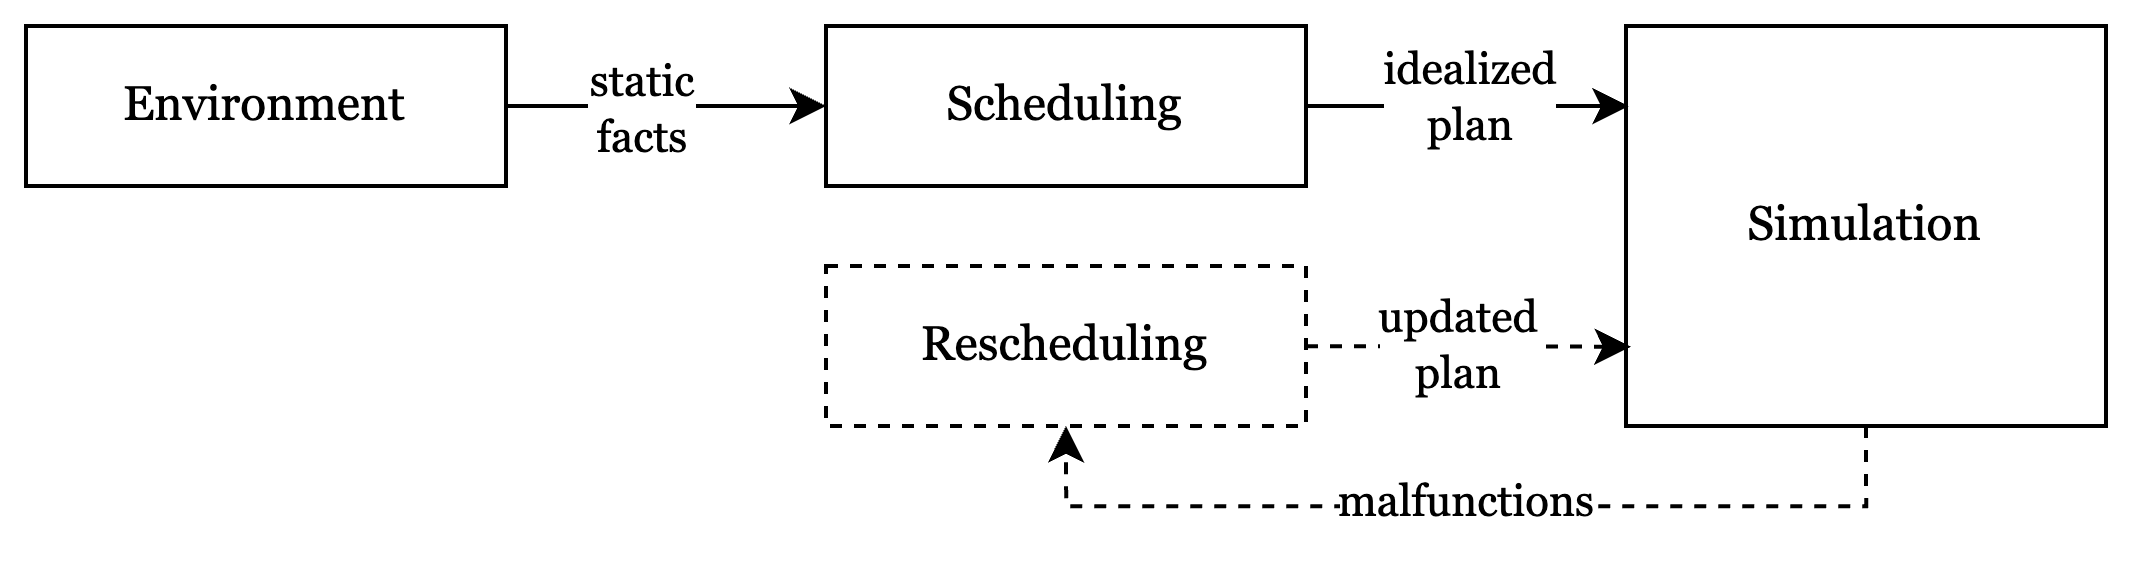
\includegraphics[width=0.8\linewidth, keepaspectratio]{figures/flowchart.png}
  \caption{Logical flow of the \textit{flaspland} system. The dashed lines represent the proposed extension to handle malfunctions}
  \label{fig:flowchart}
\end{figure}

The next significant milestone has to do with handling stochastic malfunctions.
So far, they have been overlooked.
Generally, railway routing and scheduling problems can be viewed in two stages:
\begin{enumerate}
\item \textbf{Planning.} Planning under ideal conditions is known as the vehicle scheduling problem (VSP).
\item \textbf{Execution.} Developing new plans under realistic conditions once execution has already begun is known as the vehicle rescheduling problem (VRSP).
\end{enumerate}
So far, our encodings have been well suited for the VSP,
as we pass along plans in a single-shot solving fashion.
In the future, we will need to adjust our architecture
to function as a two-way channel,
to pass forward calculated train plans,
as well as to report back changes from the simulation to our encodings,
as shown in Figure~\ref{fig:flowchart}.
Concurrently, the encodings will need to shift toward
a multi-shot solving paradigm, to account for changes in current conditions.

In principle, the logic of a VSP encoding could be recycled
by treating a the state of the simulation following a malfunction
as a \textit{fresh start} (i.e. a new environment, as if the current state of the trains were their new starting conditions),
but if conventional wisdom prevails,
benefits exist by retaining information that has already been learned.

Beyond this, my sights are set on tackling the individual problems that comprise railway systems.
We will continue to build a community of those who enroll in our railway scheduling graduate course
and those who choose to write the theses with us on this topic.

%
%%% Local Variables:
%%% mode: LaTeX
%%% TeX-master: "paper"
%%% End:

\appendix
%
\section{Source code}
\label{sec:source}

\subsection{Encodings based on directed graphs with edge transition functions}
%
% --------------------------------------------------------------------------------
\lstinputlisting[frame=single,language=clingos,firstline=8,caption={\texttt{move2drive/move-edge-functions-two.lp}}]{encodings/move2drive/move-edge-functions-two.lp}
% --------------------------------------------------------------------------------
% --------------------------------------------------------------------------------
\lstinputlisting[frame=single,language=clingos,firstline=8,caption={\texttt{move2drive/move-edge-functions-one.lp}}]{encodings/move2drive/move-edge-functions-one.lp}
% --------------------------------------------------------------------------------

\newpage

\subsection{Encodings based on directed graphs with sub-nodes}

% --------------------------------------------------------------------------------
\lstinputlisting[frame=single,language=clingos,firstline=8,caption={\texttt{move2drive/move-subnodes-two.lp}}]{encodings/move2drive/move-subnodes-two.lp}
% --------------------------------------------------------------------------------
% --------------------------------------------------------------------------------
\lstinputlisting[frame=single,language=clingos,firstline=8,caption={\texttt{move2drive/move-subnodes-one.lp}}]{encodings/move2drive/move-subnodes-one.lp}
% --------------------------------------------------------------------------------
% --------------------------------------------------------------------------------
\lstinputlisting[frame=single,language=clingos,firstline=8,caption={\texttt{drive/drive-subnodes.lp}}]{encodings/drive/drive-subnodes.lp}
% --------------------------------------------------------------------------------

% --------------------------------------------------------------------------------
% \lstinputlisting[frame=single,language=clingos,caption={\texttt{kep-routing.lp}}]{encodings/kep-routing.lp}
% --------------------------------------------------------------------------------
% --------------------------------------------------------------------------------
% \lstinputlisting[frame=single,language=clingos,caption={\texttt{kep-recursive-subnodes.lp}}]{encodings/kep-recursive-subnodes.lp}
% --------------------------------------------------------------------------------

\subsection{Encodings based on directed graphs with hyper-edges}

% --------------------------------------------------------------------------------
\lstinputlisting[frame=single,language=clingos,firstline=8,caption={\texttt{drive/drive-hyper-edges.lp}}]{encodings/drive/drive-hyper-edges.lp}
% --------------------------------------------------------------------------------
% --------------------------------------------------------------------------------
\lstinputlisting[frame=single,language=clingos,firstline=8,caption={\texttt{move2drive/move-hyper-edges.lp}}]{encodings/move2drive/move-hyper-edges.lp}
% --------------------------------------------------------------------------------

\newpage
\subsection{Path-oriented encodings}

% --------------------------------------------------------------------------------
\lstinputlisting[frame=single,language=clingos,caption={\texttt{drive.lp}}]{encodings/path2drive/drive.lp}
\lstinputlisting[frame=single,language=clingos,caption={\texttt{pathfinding-common.lp}}]{encodings/path2drive/pathfinding-common.lp}
\lstinputlisting[frame=single,language=clingos,caption={\texttt{pathfinding-edge-functions.lp}}]{encodings/path2drive/pathfinding-edge-functions.lp}
\lstinputlisting[frame=single,language=clingos,caption={\texttt{pathfinding-hypergraph.lp}}]{encodings/path2drive/pathfinding-hypergraph.lp}
\lstinputlisting[frame=single,language=clingos,caption={\texttt{pathfinding-subnodes.lp}}]{encodings/path2drive/pathfinding-subnodes.lp}
\lstinputlisting[frame=single,language=clingos,caption={\texttt{show-path.lp}}]{encodings/path2drive/show-path.lp}
% --------------------------------------------------------------------------------

%%% Local Variables:
%%% mode: LaTeX
%%% TeX-master: "paper"
%%% End:

%\bibliography{krr,procs}
%\bibliography{include/bibliography/floc}
\bibliography{local}

\end{document}

%%% Local Variables:
%%% mode: LaTeX
%%% TeX-master: t
%%% End:
